\section{Das Spektrum eines Rings}

\begin{DefBem}
Sei $R$ ein Ring.

\begin{enumerate}
\item $\Spec{R} := \{ \mathfrak{p} \subset R : \mathfrak{p} \text{ Primideal } \}$ hei\ss t \emp{Spektrum}\index{Spektrum} von $R$.

\item Eine Teilmenge $V \subseteq \Spec{R}$ hei\ss t \emp{abgeschlossen}\index{abgeschlossen}, wenn es ein Ideal $I \subseteq R$ gibt mit
$$V = V(I) = \{ \mathfrak{p} \in \Spec{R} : I \subseteq \mathfrak{p} \}$$

\item Die abgeschlossenen Teilmengen von $\Spec{R}$ definieren eine Topologie auf $\Spec{R}$, sie hei\ss t die \emp{Zariski-Topologie}\index{Zariski-Topologie}.
\end{enumerate}
\end{DefBem}

\begin{nnBsp}
$R = \ZZ$: $\Spec{\ZZ} = \{ (0) \} \cup \{ (p) : p \text{ Primzahl} \}$

$V( (p) ) = (p)$ $\Rightarrow$ $(p)$ ist abgeschlossen in $\Spec{R}$ f\"ur jede Primzahl $p$.

$V( (0) ) = \Spec{\ZZ}$.

$I = n \ZZ$ $\Rightarrow$ $V(I) = \{ (p_1), \ldots, (p_k) \}$, wenn $n = p_1^{\nu_1} \cdots p_k^{\nu_k}$ die Primfaktorzerlegung von $n$ ist.

$\overline{ \{ (0) \} } = \Spec{\ZZ}$.
\bigskip

$R = k[X]$: $\overline{ \{ (0) \} } = \Spec{R}$.

$f \in k[X]$ irreduzibel $\Rightarrow$ $(f)$ ist abgeschlossener Punkt.

$k := \CC$: $f$ irreduzibel $\Leftrightarrow$ $f(X) = X - c$ f\"ur ein $c \in
\CC$ $\Rightarrow$ $\Spec{\CC[X]} = \CC \cup \{ (0) \}$ (andere Topologie als
auf $\CC$).

\end{nnBsp}

\begin{Bew}
\begin{enumerate}
\stepcounter{enumi}
\stepcounter{enumi}
\item Sei $U \subseteq \Spec{R}$ offen :$\Leftrightarrow$ $\Spec{R} \setminus U$
abgeschlossen.

Zu zeigen:
\begin{enumerate}
\item[(i)] $\emptyset$ ist abgeschlossen: $\emptyset = V(R)$.\\
$\Spec{R}$ ist abgeschlossen: $\Spec{R} = V( (0) )$.

\item[(ii)] endliche Vereinigung von abgeschlossenen Mengen ist abgeschlossen.

Zeige dazu: $V(I_1) \cup \cdots \cup V(I_n) = V(I_1 \cap \cdots \cap I_n) = V(I_1 \cdots I_n)$

\textbf{denn:} \OE\ sei $n=2$:

\glqq$\subseteq$\grqq: Sei $\mathfrak{p} \in V(I_1)$ $\Rightarrow$ $I_1 \subseteq \mathfrak{p}$ $\Rightarrow$ $I_1 \cap I_2 \subseteq \mathfrak{p}$ $\Rightarrow$ $\mathfrak{p} \in V(I_1 \cap I_2)$.

\glqq$\supseteq$\grqq: Sei $\mathfrak{p} \in V(I_1 \cap I_2)$, $\mathfrak{p} \not\in V(I_1)$.\\
Dann gibt es ein $a \in I_1 \setminus \mathfrak{p}$. Sei $b \in I_2$.\\
Dann ist $a \cdot b \in I_1 \cap I_2 \overset{\text{Vor.}}{\subset} \mathfrak{p}$ $\overset{\substack{\mathfrak{p}\text{ prim} \\ a \notin \mathfrak{p}}}{\Rightarrow}$ $b \in \mathfrak{p}$ $\Rightarrow$ $I_2 \subseteq \mathfrak{p}$, d.h. $\mathfrak{p} \in V(I_2)$.

\item[(iii)] beliebiger Durchschnitt von abgeschlossenen Mengen ist abgeschlossen. Zeige dazu:
$$\bigcap_\nu V(I_\nu) = V\left(\sum_\nu I_\nu\right)$$

\textbf{denn:} $\mathfrak{p} \in \bigcap_\nu V(I_\nu)$ $\Leftrightarrow$ $I_\nu \subseteq \mathfrak{p}\ \forall \nu$ $\Leftrightarrow$ $\sum_\nu I_\nu \subseteq \mathfrak{p}$.

\end{enumerate}
\end{enumerate} 

\end{Bew}



\begin{Bem}

\begin{enumerate}
\item F\"ur Ideale $I_1 \subseteq I_2$ ist $V(I_1) \supseteq V(I_2)$.

\item F\"ur jedes Ideal $I \subseteq R$ ist $V(I) = V(\sqrt{I}) = V(\Rad{I})$

\item
Die $U(f) := \Spec{R}\setminus V( (f) )$, $f \in R \setminus \sqrt{(0)}$ bilden
eine Basis der Zariski-Topologie.

\begin{Bew}
\textbf{Zusatz:} $U(f) = \{ \mathfrak{p} \in \Spec{R} : f \notin \mathfrak{p} \}$.

\end{Bew}

\end{enumerate}

\end{Bem}

\begin{Bew}
\begin{enumerate}
\item Sei $\mathfrak{p}$ Primideal mit $I \subseteq \mathfrak{p}$, $f \in
\sqrt{I}$, dann ist $f^n \in I$ f\"ur ein $n \geq 1$. $\Rightarrow$ $f^n \in
\mathfrak{p}$ $\underset{\mathfrak{p} \text{ prim}}\Rightarrow$ $f \in
\mathfrak{p}$ $\Rightarrow$ $\sqrt{I} \subseteq \mathfrak{p}$.
\item 
$\sqrt{(0)} = \bigcap_{\mathfrak{p} \in \Spec{R}}{\mathfrak{p}}$ (\"U7A2b)

Also ist $V(f) = \Spec{R}$ $\Leftrightarrow$ $f \in \sqrt{(0)}$. F\"ur $f \in R \setminus \sqrt{(0)}$ ist also $U(f) \neq \emptyset$.

Zu zeigen: Ist $U \subseteq \Spec{R}$ offen, $U \neq \emptyset$, so gibt es ein $f \in R \setminus \sqrt{(0)}$ mit $U(f) \subseteq U$.

Sei also $U = \Spec{R}\setminus V(I)$ mit $I \nsubseteq \sqrt{(0)}$. F\"ur $f
\in I \setminus \sqrt{(0)}$ ist $(f) \subseteq I$, also $V(f) \supseteq V(I)$
$\Rightarrow$ $U(f) \subseteq U$. 
\end{enumerate}
\end{Bew}

\begin{DefProp}

\begin{enumerate}
\item Ein topologischer Raum $X$ heißt \emp{irreduzibel}\index{irreduzibel}, wenn er nicht Vereinigung zweier echter abgeschlossener Teilmengen ist.

\begin{nnBsp}
$R = \CC[X,Y]$,\\
$V((X)) = \{ (X) \} \cup \{ (X, Y - c), c \in \CC \}$\\
$V((Y)) = \{ (Y) \} \cup \{ (X -a, Y), a \in \CC \}$.

$V((X \cdot Y)) = V( (X) ) \cup V( (Y) )$ = Achsenkreuz
% TODO Zeichnung -> habs versucht, sagt aber nicht viel aus :-/
\end{nnBsp}

\item Eine abgeschlossene Teilmenge $V(I) \subseteq \Spec{R}$ ist genau dann irreduzibel, wenn $I$ ein Primideal ist.

\begin{Bew}
\glqq$\Rightarrow$\grqq: Seien $f_1, f_2 \in R$, $f_1 \cdot f_2 \in I$ und $f_1 \notin I$. Dann ist $V((f_1)) \nsupseteq V := V(I)$.

Andererseits: $V \subseteq V((f_1 \cdot f_2)) = V((f_1)) \cup V((f_2))$\\
$\Rightarrow$ $V = (V \cap V((f_1))) \cup (V \cap V((f_2)))$\\
$\overset{V \text{ irreduz.}}\Rightarrow$ $V \subseteq V((f_2))$ $\Rightarrow$ $f_2 \in I$.

\glqq$\Leftarrow$\grqq: Sei $V(I) = V = V(I_1) \cup V(I_2)$ und $V(I_1) \neq V$

d.h. $I_1 \nsubseteq I$. Sei $f_1 \in I_1 \setminus I$.

Andererseits ist $V(I_1 \cdot I_2) = V(I_1) \cup V(I_2) = V$ $\Rightarrow$ $I_1 \cdot I_2 \subseteq \sqrt{I} = I$.

F\"ur jedes $f \in I_2$ ist also $f_1 \cdot f \in I$ $\overset{f_1 \notin I}\Rightarrow$ $f \in I$ $\Rightarrow$ $I_2 \subseteq I$ $\Rightarrow$ $V(I) \subseteq V(I_2)$.

\end{Bew}

\end{enumerate}

\end{DefProp}

\begin{Folg}
Ist $\Spec{R}$ hausdorffsch, so ist $\dim R = 0$.

\begin{Bew}
$\Spec{R}$ hausdorffsch $\Rightarrow$ jede irreduzible Teilmenge von
$\Spec{R}$ ist einelementig, denn für $X\subseteq\Spec{R}$ ist
\[
X=(X\setminus U)\cup(X\setminus V)
\]
eine echte Zerlegung in abgeschlossene
Teilmengen.

\begin{center}
	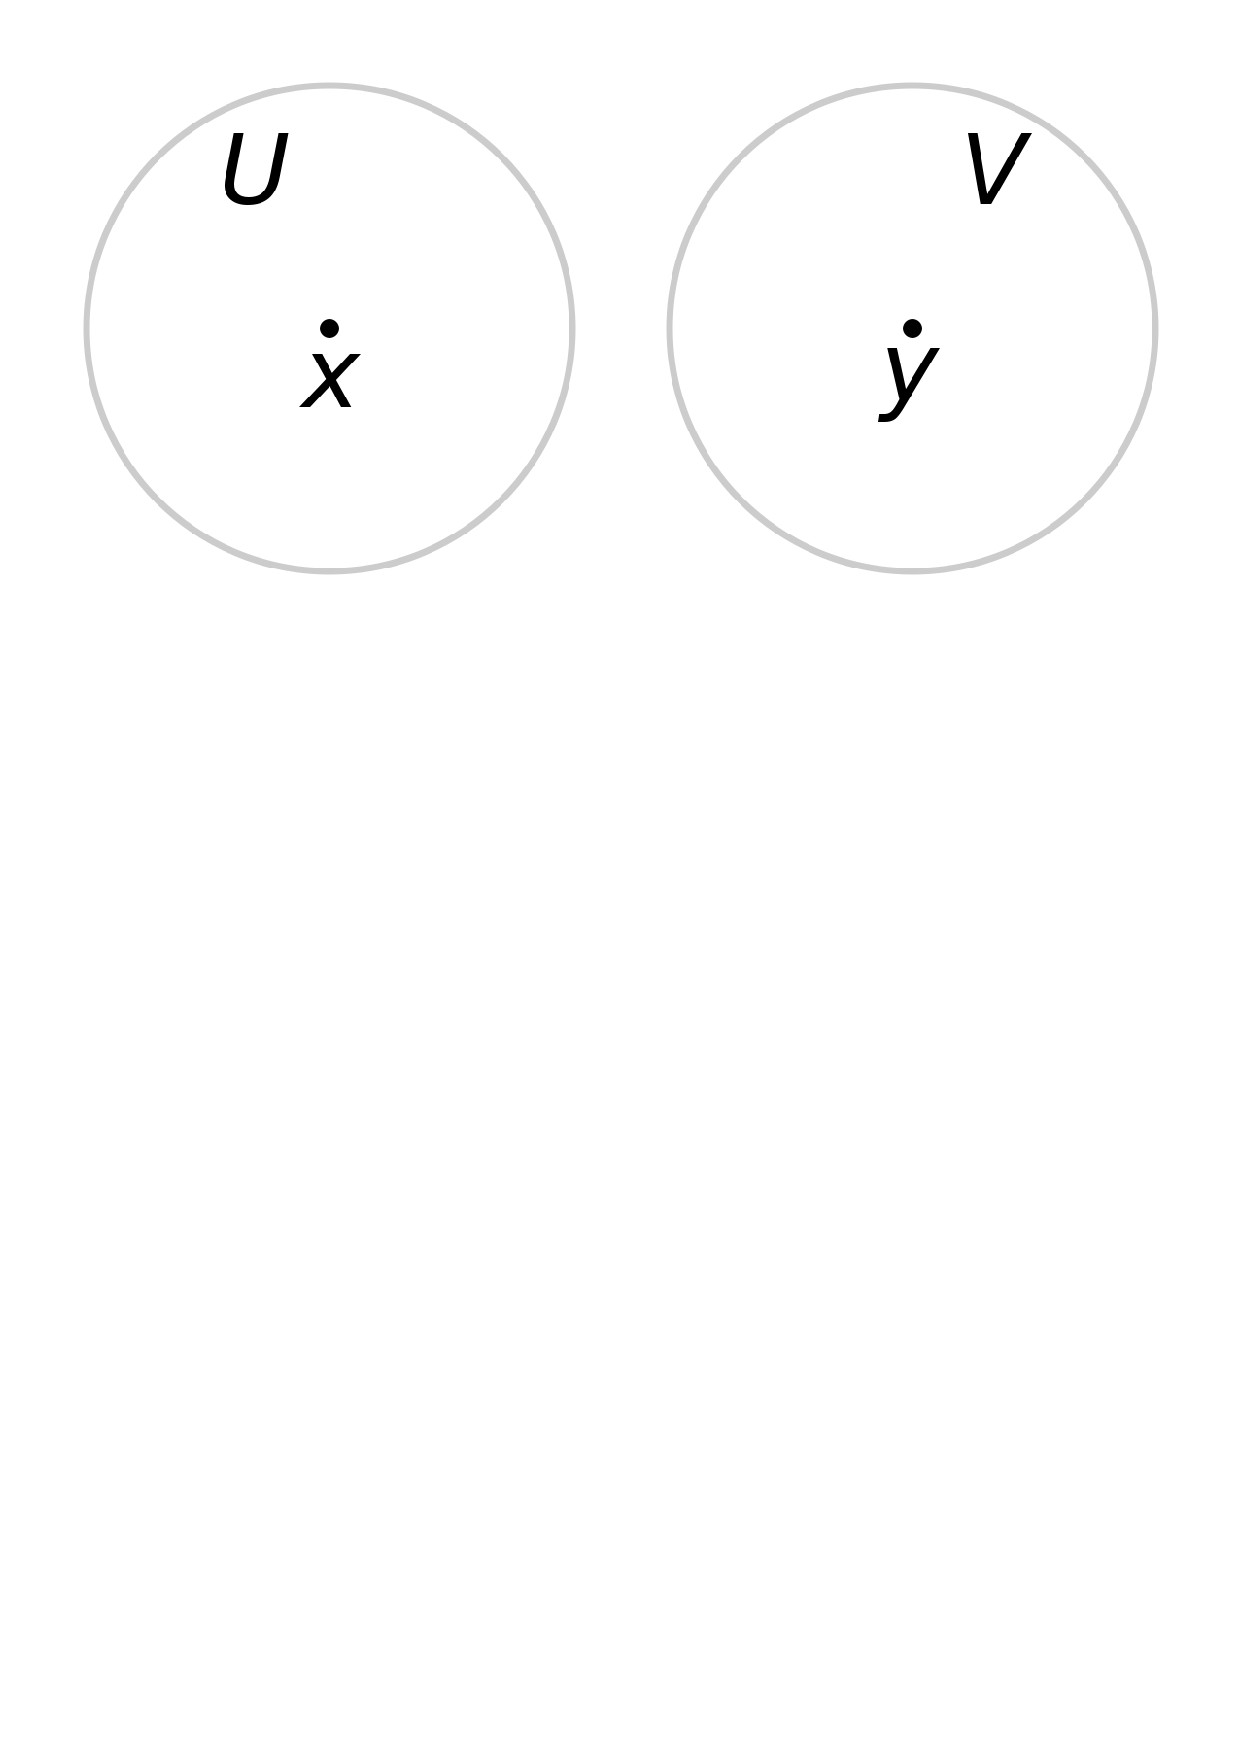
\includegraphics[width=0.75\textwidth]{images/algebra2/hausdorff.pdf}
\end{center}

$\Rightarrow$ F\"ur jedes Primideal $\mathfrak{p}$ von $R$ ist $V(\mathfrak{p}) = \{ \mathfrak{p} \}$

$\Rightarrow$ jedes Primideal in $R$ ist maximales Ideal

$\Rightarrow$ $\dim R = 0$.

\end{Bew}

\end{Folg}

\begin{DefBem}

\begin{enumerate}
\item F\"ur eine beliebige Teilmenge $V$ von $\Spec{R}$ hei\ss t $$\displaystyle I(V) = \bigcap_{\mathfrak{p} \in V} \mathfrak{p}$$ das \emp{Verschwindungsideal}\index{Verschwindungsideal} von $V$.

\item F\"ur jedes Ideal $I$ von $R$ gilt:
$$I(V(I)) = \sqrt{I}$$

\begin{Bew}
Nach \"U7A2d ist $\displaystyle \sqrt{I} = \bigcap_{\substack{\mathfrak{p} \supseteq I \\ \mathfrak{p} \text{ Primideal}}} \mathfrak{p} = \bigcap_{\mathfrak{p} \in V(I)} \mathfrak{p}$
\end{Bew}

\end{enumerate}

\end{DefBem}

\begin{nnFolg}
Ist $V(I_1) = V(I_2)$, so ist $\sqrt{I_1} = \sqrt{I_2}$.
\end{nnFolg}

\begin{DefProp}
\begin{enumerate}
\item Sei $X$ ein topologischer Raum. Eine irreduzible Teilmenge $V \subseteq X$ hei\ss t \emp{irreduzible Komponente}\index{irreduzible Komponente}, wenn $V$ maximale irreduzible Teilmenge ist.

\item Jeder topologischer Raum ist Vereinigung seiner irreduziblen Komponenten.

\item Ist $R$ noethersch, so ist jede abgeschlossene Teilmenge von $V$ von $\Spec{R}$ endliche Vereinigung von irreduziblen Komponenten von $V$; diese sind eindeutig bestimmt.

\end{enumerate}

\begin{Bew}
\begin{enumerate}

\item Zu zeigen: jedes $x \in X$ ist in einer irreduziblen Teilmenge von $X$ enthalten.

Sei $\mathcal{C}_x := \{ U \subseteq X : x \in U, U \text{ irreduzibel} \}$.

$\mathcal{C}_x \neq \emptyset$, da $\{ x \} \in \mathcal{C}_x$.

Seien $(U_i)_{i \in \NN}$ in $\mathcal{C}_x$ mit $U_i \subseteq U_{i+1}$ f\"ur alle $i$.

Sei $U := \bigcup_{i \in \NN} U_i$, zu zeigen: $U \in \mathcal{C}_x$, d.h. $U$ irreduzibel.

\textbf{denn:} Sei $U = V \cup W$, $V,W$ abgeschlossene Teilmengen von $U$. Dann ist $U_i = (U_i \cap V) \cup (U_i \cap W)$ f\"ur jedes $i \in \NN$

Da $U_i$ irreduzibel, ist (\OE) $U_i \cap V = U_i$ f\"ur unendliche viele $i$.

$\Rightarrow$ $U_i \subseteq V$ $\Rightarrow$ $U = \bigcup_{\text{diese }i} U_i \subseteq V$ $\Rightarrow$ $U \subseteq V$.

$\Rightarrow$ $U$ irreduzibel.

Mit dem Zornschen Lemma folgt: $\mathcal{C}_x$ enth\"alt ein maximales Element.

\item \OE\ sei $V = \Spec{R}$: Sei $V = V(I)$ f\"ur ein Ideal $I$.

$V(I) = \{ \mathfrak{p} \in \Spec{R} : I \subseteq \mathfrak{p} \} \overset{\text{bijektiv}}\longleftrightarrow \{ \mathfrak{p'} \in \Spec{R/I} \}$

Aus 2.34b wird folgen: Die Abbildung ist ein Hom\"oomorphismus.

Sei $\mathfrak{V}$ die Menge der abgeschlossenen Teilmengen von $\Spec{R}$, die
\underline{nicht} Vereinigung von endlich vielen irreduziblen Teilmengen sind.
Weiter sei $J := \{ I(V) : V \in \mathfrak{V} \}$.

Zu zeigen: $\mathfrak{V} = \emptyset$.

Anderenfalls ist auch $J \neq \emptyset$. Da $R$ noethersch ist, enth\"alt $J$ ein maximales Element $I(V_0)$ f\"ur ein $V_0 \in \mathfrak{V}$.

$V_0$ ist nicht irreduzibel.

Also gibt es abgeschlossene Teilmengen $V_1, V_2$ von $V_0$ mit $V_0 = V_1 \cup V_2$, $V_1 \neq V_0 \neq V_2$.

$V_i \notin \mathfrak{V}$ f\"ur $i = 1,2$, da $I(V_0) \subsetneqq I(V_i)$

Also lassen sich $V_1$ und $V_2$ als endliche Vereinigung von irreduziblen Teilmengen schreiben.

$\Rightarrow$ $V_0$ l\"asst sich auch als endliche Vereinigung von irreduziblen Teilmengen schreiben. Widerspruch zur Wahl von $V_0$.

$\Rightarrow$ $\mathfrak{V} = \emptyset$.
\bigskip

Sei also $V = V_0 \cup \cdots \cup V_r$ mit irreduziblen Teilmengen $V_i$.

Noch zu zeigen: 
\begin{itemize}
\item die $V_i$ sind (\OE) irreduzible Komponenten.
\item Eindeutigkeit
\end{itemize}

\textbf{denn:}

Aus b) folgt: jedes $V_i$ ist in einer irreduziblen Komponente
$\widetilde{V_i}$ von $V$ enthalten, also $V = \bigcup_{i=0}^r
\widetilde{V_i}$; \OE\ alle $\widetilde{V_i}$ verschieden.

Sei W irreduzible Komponente von $V$.

$\Rightarrow$ $W = \bigcup_{i=0}^r (W \cap \widetilde{V_i})$ $\overset{W \text{ irreduz.}}\Rightarrow$ es gibt ein $i$ mit $W \subseteq \widetilde{V_i}$

$\overset{W \text{ Komponente}}\Rightarrow$ $W = \widetilde{V_i}$.

\end{enumerate}
\end{Bew}

\end{DefProp}

\begin{Folg}
Ein noetherscher Ring hat nur endlich viele minimale Primideale.

\begin{Bew}
Sei $\mathfrak{p} \in \Spec{R}$ minimales Primideal. $\Leftrightarrow$ $V(\mathfrak{p}) \subseteq \Spec{R}$ irreduzible Komponente.
\end{Bew}
\end{Folg}

\begin{Prop}
Sei $\alpha : R \rightarrow S$ Ringhomomorphismus.

\begin{enumerate}
\item Die Abbildung $\varphi_\alpha : \Spec{S} \rightarrow \Spec{R}$, $\mathfrak{p} \mapsto \alpha^{-1}(\mathfrak{p})$ ist stetig.

Eleganter: $R \rightarrow \Spec{R}$ ist kontravarianter Funktor
\[
\KatRing \to \KatTop.
\]

\item Ist $\alpha$ surjektiv, so ist $\varphi_\alpha$ injektiv und $\varphi_\alpha(\Spec{S}) = V(\K{\alpha})$.
\end{enumerate}

\begin{Bew}
\begin{enumerate}
\item $\alpha^{-1}(\mathfrak{p})$ ist Primideal:

Seien $a,b \in R$ mit $a \cdot b \in \alpha^{-1}(\mathfrak{p})$ $\Rightarrow$ $\alpha(a \cdot b) \in \mathfrak{p}$ $\overset{\text{\OE}}\Rightarrow$ $\alpha(a) \in \mathfrak{p}$ $\Rightarrow$ $a \in \alpha^{-1}(\mathfrak{p})$

\textbf{$\varphi_\alpha$ stetig}: Zu zeigen: f\"ur jede abgeschlossene Teilmenge $V = V(I)$ von $\Spec{R}$ ist $\varphi_\alpha^{-1}(V)$ abgeschlossen in $\Spec{S}$.

$\varphi_\alpha^{-1}(V(I)) = \{ \mathfrak{p} \in \Spec{S} : I \subseteq
\alpha^{-1}(\mathfrak{p}) \} = \{ \mathfrak{p} \in \Spec{S} : \alpha(I)
\subseteq \mathfrak{p} \} = \{ \mathfrak{p} \in \Spec{S} : \alpha(I) \cdot S
\subseteq \mathfrak{p} \} = V(\alpha(I) \cdot S)$.

\item
Seien $\mathfrak{p}, \mathfrak{p'} \in \Spec{S}$ mit $\varphi_\alpha(\mathfrak{p}) = \varphi_\alpha(\mathfrak{p'})$

$\Rightarrow$ $\alpha^{-1}(\mathfrak{p}) = \alpha^{-1}(\mathfrak{p'})$

$\Rightarrow$ $\alpha(\alpha^{-1}(\mathfrak{p})) = \alpha(\alpha^{-1}(\mathfrak{p'}))$

$\overset{\alpha \text{ surj.}}\Rightarrow$ $\mathfrak{p} = \mathfrak{p'}$.

\end{enumerate}
\end{Bew}
\end{Prop}
